\let\negmedspace\undefined
\let\negthickspace\undefined
%\RequirePackage{amsmath}
\documentclass[journal,12pt,twocolumn]{IEEEtran}
%
% \usepackage{setspace}
\usepackage{gensymb}
%\doublespacing
%\singlespacing
%\usepackage{silence}
%Disable all warnings issued by latex starting with "You have..."
%\usepackage{graphicx}
\usepackage{amssymb}
%\usepackage{relsize}
\usepackage[cmex10]{amsmath}
%\usepackage{amsthm}
%\interdisplaylinepenalty=2500
%\savesymbol{iint}
%\usepackage{txfonts}
%\restoresymbol{TXF}{iint}
%\usepackage{wasysym}
\usepackage{amsthm}
%\usepackage{pifont}
%\usepackage{iithtlc}
% \usepackage{mathrsfs}
% \usepackage{txfonts}
\usepackage{stfloats}
% \usepackage{steinmetz}
\usepackage{bm}
% \usepackage{cite}
% \usepackage{cases}
% \usepackage{subfig}
%\usepackage{xtab}
\usepackage{longtable}
%\usepackage{multirow}
%\usepackage{algorithm}
%\usepackage{algpseudocode}
\usepackage{enumitem}
\usepackage{mathtools}
\usepackage{tikz}
% \usepackage{circuitikz}
% \usepackage{verbatim}
%\usepackage{tfrupee}
\usepackage[breaklinks=true]{hyperref}
%\usepackage{stmaryrd}
%\usepackage{tkz-euclide} % loads  TikZ and tkz-base
%\usetkzobj{all}
\usepackage{listings}
\usepackage{color}                                            %%
\usepackage{array}                                            %%
\usepackage{longtable}                                        %%
\usepackage{calc}                                             %%
\usepackage{multirow}                                         %%
\usepackage{hhline}                                           %%
\usepackage{ifthen}                                           %%
%optionally (for landscape tables embedded in another document): %%
\usepackage{lscape}     
% \usepackage{multicol}
% \usepackage{chngcntr}
%\usepackage{enumerate}

%\usepackage{wasysym}
%\newcounter{MYtempeqncnt}
\DeclareMathOperator*{\Res}{Res}
\DeclareMathOperator*{\equals}{=}
%\renewcommand{\baselinestretch}{2}
\renewcommand\thesection{\arabic{section}}
\renewcommand\thesubsection{\thesection.\arabic{subsection}}
\renewcommand\thesubsubsection{\thesubsection.\arabic{subsubsection}}

\renewcommand\thesectiondis{\arabic{section}}
\renewcommand\thesubsectiondis{\thesectiondis.\arabic{subsection}}
\renewcommand\thesubsubsectiondis{\thesubsectiondis.\arabic{subsubsection}}

% correct bad hyphenation here
\hyphenation{op-tical net-works semi-conduc-tor}                 

\lstset{
	%language=C,
	frame=single, 
	breaklines=true,
	columns=fullflexible
}
%\lstset{
	%language=tex,
	%frame=single, 
	%breaklines=true
	%}

\begin{document}
	
	%


\newtheorem{theorem}{Theorem}[section]
\newtheorem{problem}{Problem}
\newtheorem{proposition}{Proposition}[section]
\newtheorem{lemma}{Lemma}[section]
\newtheorem{corollary}[theorem]{Corollary}
\newtheorem{example}{Example}[section]
\newtheorem{definition}[problem]{Definition}
%\newtheorem{thm}{Theorem}[section] 
%\newtheorem{defn}[thm]{Definition}
%\newtheorem{algorithm}{Algorithm}[section]
%\newtheorem{cor}{Corollary}
\newcommand{\BEQA}{\begin{eqnarray}}
	\newcommand{\EEQA}{\end{eqnarray}}
\newcommand{\define}{\stackrel{\triangle}{=}}
\newcommand*\circled[1]{\tikz[baseline=(char.base)]{
		\node[shape=circle,draw,inner sep=2pt] (char) {#1};}}
\bibliographystyle{IEEEtran}
%\bibliographystyle{ieeetr}


\providecommand{\mbf}{\mathbf}
\providecommand{\pr}[1]{\ensuremath{\Pr\left(#1\right)}}
\providecommand{\qfunc}[1]{\ensuremath{Q\left(#1\right)}}
\providecommand{\sbrak}[1]{\ensuremath{{}\left[#1\right]}}
\providecommand{\lsbrak}[1]{\ensuremath{{}\left[#1\right.}}
\providecommand{\rsbrak}[1]{\ensuremath{{}\left.#1\right]}}
\providecommand{\brak}[1]{\ensuremath{\left(#1\right)}}
\providecommand{\lbrak}[1]{\ensuremath{\left(#1\right.}}
\providecommand{\rbrak}[1]{\ensuremath{\left.#1\right)}}
\providecommand{\cbrak}[1]{\ensuremath{\left\{#1\right\}}}
\providecommand{\lcbrak}[1]{\ensuremath{\left\{#1\right.}}
\providecommand{\rcbrak}[1]{\ensuremath{\left.#1\right\}}}
\theoremstyle{remark}
\newtheorem{rem}{Remark}
\newcommand{\sgn}{\mathop{\mathrm{sgn}}}
\providecommand{\abs}[1]{\left\vert#1\right\vert}
\providecommand{\res}[1]{\Res\displaylimits_{#1}} 
\providecommand{\norm}[1]{\left\lVert#1\right\rVert}
%\providecommand{\norm}[1]{\lVert#1\rVert}
\providecommand{\mtx}[1]{\mathbf{#1}}
\providecommand{\mean}[1]{E\left[ #1 \right]}
\providecommand{\fourier}{\overset{\mathcal{F}}{ \rightleftharpoons}}
%\providecommand{\hilbert}{\overset{\mathcal{H}}{ \rightleftharpoons}}
\providecommand{\system}{\overset{\mathcal{H}}{ \longleftrightarrow}}
%\newcommand{\solution}[2]{\textbf{Solution:}{#1}}
\newcommand{\solution}{\noindent \textbf{Solution: }}
\newcommand{\cosec}{\,\text{cosec}\,}
\providecommand{\dec}[2]{\ensuremath{\overset{#1}{\underset{#2}{\gtrless}}}}
\newcommand{\myvec}[1]{\ensuremath{\begin{pmatrix}#1\end{pmatrix}}}
\newcommand{\mydet}[1]{\ensuremath{\begin{vmatrix}#1\end{vmatrix}}}
%\numberwithin{equation}{section}
\numberwithin{equation}{subsection}
%\numberwithin{problem}{section}
%\numberwithin{definition}{section}
\makeatletter
\@addtoreset{figure}{problem}
\makeatother

\let\StandardTheFigure\thefigure
\let\vec\mathbf
%\renewcommand{\thefigure}{\theproblem.\arabic{figure}}
\renewcommand{\thefigure}{\theproblem}
%\setlist[enumerate,1]{before=\renewcommand\theequation{\theenumi.\arabic{equation}}
	%\counterwithin{equation}{enumi}
	
	
	%\renewcommand{\theequation}{\arabic{subsection}.\arabic{equation}}
	
	\def\putbox#1#2#3{\makebox[0in][l]{\makebox[#1][l]{}\raisebox{\baselineskip}[0in][0in]{\raisebox{#2}[0in][0in]{#3}}}}
	\def\rightbox#1{\makebox[0in][r]{#1}}
	\def\centbox#1{\makebox[0in]{#1}}
	\def\topbox#1{\raisebox{-\baselineskip}[0in][0in]{#1}}
	\def\midbox#1{\raisebox{-0.5\baselineskip}[0in][0in]{#1}}
	
	\vspace{3cm}

	\textbf{ICSE class 12 paper 2018}
	\section{Question 20(a)} 
Find the line of regression of y on x from the following table.
Hence, estimate the y value when x=6.
	\begin{table}[h!]
		\resizebox{\columnwidth}{!} {
			\begin{tabular}{|c|c|c|c|c|c|}
				\hline
				x &1 &2&3 & 4& 5 \\
				\hline
				y &7 & 6 & 5 &4 & 3\\
				\hline
			\end{tabular}
		}
	\end{table}

	
	\textbf{Solution.}
	
	
	Given observations
	\begin{align}
		 \myvec{x_1\\y_1},\myvec{x_2\\y_2}.....,\myvec{x_n\\y_n}
	\end{align}
	Best fit a straight line to it , $e_i$ are the corresponding residual errors,coeffients $a_0$and $a_1$
	      \begin{align}   
	      	\vec{Y}&=\myvec{y_1\\y_2\\.\\.\\y_{n-1}\\y_n},
	      	\vec{X}=\myvec{1&x_1\\1&x_2\\.&\\.&\\1&x_{n-1}\\1&x_n}
	      	\\
	      	\vec{A}&=\myvec{a_1\\a_0},
	      	\vec{E}=\myvec{e_1\\e_2\\.\\.\\e_{n-1}\\e_n}\\
      		\vec{E}=&\vec{Y}-\vec{X}\vec{A}
      	\end{align}
SSE is sum of square of errors , substitue E from above equation and get A
      \begin{align}
      	SSE&=\norm{\vec{E}^{\top}\vec{E}}\\ &=\brak{\vec{Y}-\vec{X}\vec{A}}^{\top}\brak{\vec{Y}-\vec{X}\vec{A}}\\
      	&=\brak{\vec{Y}^{\top}-\vec{A}^{\top}\vec{X}^{\top}}\brak{\vec{Y}-\vec{X}\vec{A}}
      	\\
      	&=\brak{\vec{Y}^{\top}\vec{Y}-2\vec{A}^{\top}\vec{X}^{\top}\vec{Y}+\vec{A}^{\top}\vec{X}^{\top}\vec{X}\vec{A}}
      	      \end{align}
            for minimizing use gradient wrt A
      	\begin{align}
      	 \nabla
      		SSE
      		&=\brak{\nabla\vec{Y}^{\top}\vec{Y}-2\nabla\vec{A}^{\top}\vec{X}^{\top}\vec{Y}+\nabla\vec{A}^{\top}\vec{X}^{\top}\vec{X}\vec{A}}\\
      		&=2\brak{\vec{X}^{\top}\vec{X}\vec{A}-\vec{X}^{\top}\vec{Y}}
      	\end{align}
      We now set this to zero at the optimum
      \begin{align}
       \brak{\vec{X}^{\top}\vec{X}\vec{A}-\vec{X}^{\top}\vec{Y}}=0\\
       \vec{A}=\brak{\vec{X}^{\top}\vec{X}}^{-1}\vec{X}^{\top}\vec{Y}
      \end{align}

  If we want to give line form after finding A
  \begin{align}
  	\vec{n}^{\top}\vec{x}=c, \vec{n}=\myvec{\vec{A}^{\top}\myvec{-1\\0}\\1},c=\vec{A}^{\top}\myvec{0\\1}
  \end{align}
	For this problem 
	\begin{align}
		\myvec{x \\y }:
	\myvec{1 \\7 },
	\myvec{2 \\6 },
	\myvec{3 \\5 },
    \myvec{4 \\4 },
    \myvec{5 \\3 }
	\end{align}
\begin{align}
	\vec{Y}=\myvec{7\\6\\5\\4\\3},
	\vec{X}=\myvec{1&1\\1&2\\1&3\\1&4\\1&5}
\end{align}
Substitue these Y and X and get A 
\begin{align}
	A=\myvec{-1\\8}
\end{align}
	After using the line form stated before
	\begin{align}
		y=8-x\\
		x+y=8
	\end{align}
	When $x=6$ then y must be 2 from the line of regression.
	
	\begin{figure}[h!]
		\centering
		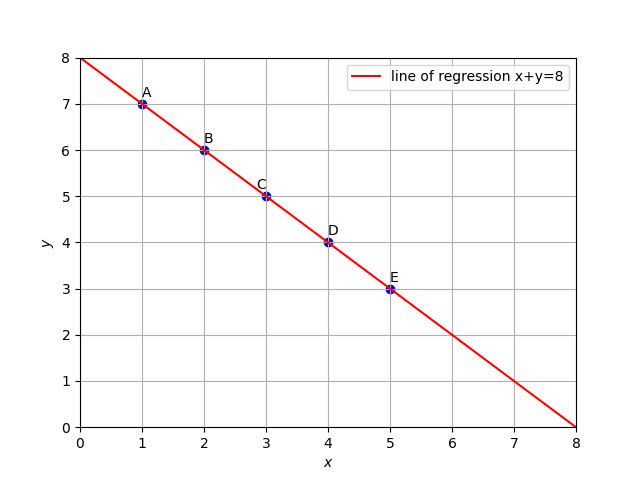
\includegraphics[width=\columnwidth]{./figs/fig1.png}
		\caption{plot of all points}
		\label{Fig1}
	\end{figure}
	
\end{document}